\documentclass[12pts]{article}

\usepackage[margin=1in]{geometry}
\usepackage[usenames, dvipsnames]{color}
\usepackage{setspace}
\usepackage{graphicx}
\doublespacing
\usepackage{fancyvrb}
\usepackage{varwidth}
\usepackage{verbatim}
\usepackage{multicol}
\usepackage{hyperref}

\usepackage{parskip}                    % This packages sets the spacing between two paragraphs
\setlength{\parskip}{.5\baselineskip}   % Define spacing between two paragraphs

\setlength{\parindent}{0pt}
\setlength{\columnseprule}{1pt}

\usepackage{fancyhdr}

\title{DIME DYNAMIC DOCUMENTATION TRAINING }
\author{Luiza Andrade \& Mrijan Rimal} 
\date{\today}


\makeatother


\begin{document}
	
	
	\makeatletter
	\begin{titlepage}
		\begin{center}
			
\includegraphics[width=0.3\linewidth]{../img/i2i.png}\\[10ex]
			{\LARGE \bfseries  \@title }\\[2ex] 
			{\Large  \@author}\\[20ex] 
			{\large \@date}
		\end{center}
		\vspace{5cm}
		\textcolor{red}{For the most recent version of this file, please check \url{https://github.com/worldbank/DIME-LaTeX-Templates/}}
	\end{titlepage}
	\makeatother
	
	\tableofcontents
	
	\newpage
	\section*{Introduction}
	This exercise is an introduction to the concepts needed to create a docuement with tables and figures outputted in {\LaTeX} from, for example, Stata or R. After this exercise you will be able to create a document that is automatically updated each time the code in Stata or R is updated and run again. The document this exercise generates is meant to be either an appendix of tables and graphs, or a document with initial results that updates instantly.
	
	For this first exercise, all the outputed tables and graphs that you need to create the document are provided for you. In later exercises you will produce them yourself.
	
	If you want to have a more broad understanding of {\LaTeX} or explore other functionalities, this \href{https://en.wikibooks.org/wiki/LaTeX
	}{{\LaTeX} Wikibook} is a great source. For more specific questions about how to perform a task or solve an error, Google usually has the answer. However, the exercises following this one will introduce you to more functionalities in {\LaTeX}.
	
	Exercise overview:
	\begin{itemize}
		\item Part 1 and 2 explains concepts often confusing to someone new to {\LaTeX}.
		\item Part 3 to 6 imports figures and tables and introduces some basic formatting.
		\item Part 7 and 8 introduces document titles and list of tables and figures.
	\end{itemize}
	
	\section{Folders and relative file paths}
	{\LaTeX} uses what is called relative file paths. We will explain what this means and while it is not complex, it is important to understand it well when working in {\LaTeX}. Start by looking in the folder where you found this handout. 
	
	In this folder, you see a folder called \emph{Output.tex} with two sub-folders, \emph{Raw} and \emph{Final}. In the \emph{Final} sub-folder, you will find a file called \emph{Exercise 1.tex}. This is the file you will be working in. We will call it the main document and you will import the tables and graphs we have provided for you to this main document file. You will also find a folder called \emph{Raw}. In this folder you will find the tables and graphs you will use in this exercise and that we have provided for you. The relative file path from \emph{Exercise 1.tex} to, for example, image \emph{iegraph.png} in the \emph{Raw} folder is therefore \verb|{../Raw/iegraph.png}|. Note that to a relative file path it does not matter where the file is stored on the computer(for example, on C drive, My Documents, the Drop-Box folder, Desktop etc). It only matters where a file is saved in relation to the starting point. The starting point in {\LaTeX} is the folder where the main document is saved. In the case of this exercise that is the folder where \emph{Exercise 1.tex} is saved.
	
	So this path \verb|{../Raw/iegraph.png}| means that, starting to the \emph{Final} folder where our main document is, first {\LaTeX} will go its parent folder (that is what the double dots do), and then look there for another folder called \emph{Raw}, and from that folder open a file called \emph{iegraph.png}. The file path \verb|{iegraph.png}| on the other hand means that the graph would be saved directly in the same folder as the main document. This is usually bad practice as when your document grows it will reference a lot of files and storing all those files in a sub-folder is much cleaner way to organize the files. Relative file paths can be multiple folders deep, for example \verb|{../Raw/baseline/income_chapter/iegraph.png}|. 
	
	Relative file paths are very simple as long as the files referenced are stored in close relation to the main document, but this is soon obvious to you unless it already is.
	
	\section{Compiling a pdf file from  {\LaTeX} code}
	In {\LaTeX}, compiling means that you run your code to create and save a pdf version of your document. It is similar to running a do-file in Stata or an R-script in R but it creates a pdf instead of running computations. 
	
	In TeXstudio, open the file \emph{Exercise 1.tex} that you find in the folder for this exercise. This is a very basic {\LaTeX} document and consists on the initial settings we will build on. The preamble at the top of the document loads different functionalities that we will be using, but you do not have to worry about this until later exercises.
	
	To compile the document go to \emph{Tools} in the top drop-down menu in TeXstudio when you have the code in \emph{Exercise 1.tex} open. Then click \emph{Compile}, but you wont to see anything happening. Instead, click \emph{Build \& View} in the \emph{Tools} menu. This should open a new window in TeXstudio where you see the text \emph{This is a blank document}. Both \emph{Compile} and \emph{Build \& View} creates a pdf and saves it to disk, but only \emph{Build \& View} opens up a window where you can see your document directly. 
	
	The pdf file was saved in the same folder as where the file \emph{Exercise 1.tex} is saved. {\LaTeX} exports a lot of auxiliary files as well here. You do not need these files. It is possible to have these files saved elsewhere, but do not worry about that now, and most {\LaTeX} users never bother to change where those files are saved.
	
	If you open the \emph{Tools} menu again you can see short cuts for next time you want to compile your document. You can click \emph{F5} to \emph{Build \& View} and \emph{F6} to \emph{Compile}. You also see two icons that look like green play-buttons. You can find the same icons in the bar underneath the drop-down menus. Most {\LaTeX} users use either of those two short cuts.
	
	\section{Using TeXstudio interface to import an image into \LaTeX}
	Now it is time to start importing some files into our document. Make sure that you still have \emph{Exercise 1.tex} open. Again, do not worry about the preamble, for the rest of this exercise, you will only add lines of code between \verb|\begin{document}| and \verb|end{document}| to create your document content.
	
	We first want to show you a short cut that you can use to import files to your document that you can use until you feel confident in using relative file paths. While you keep \emph{Exercise 1.tex} open in TeXstudio, open the \emph{Raw} folder in regular Explorer (Windows) or Finder (Mac) window. Now click \emph{take\_up.png} and drag it to the part of \emph{Exercise 1.tex} that says ``This is a blank document". Then click ``OK" in the window that pops up. This will create a section of code that should look similar to the code below. Now, compile your document using \emph{Build \& View}.
	
	\begin{center}
		\begin{Verbatim}[commandchars=+\(\)]
		\begin{figure}
			\centering
			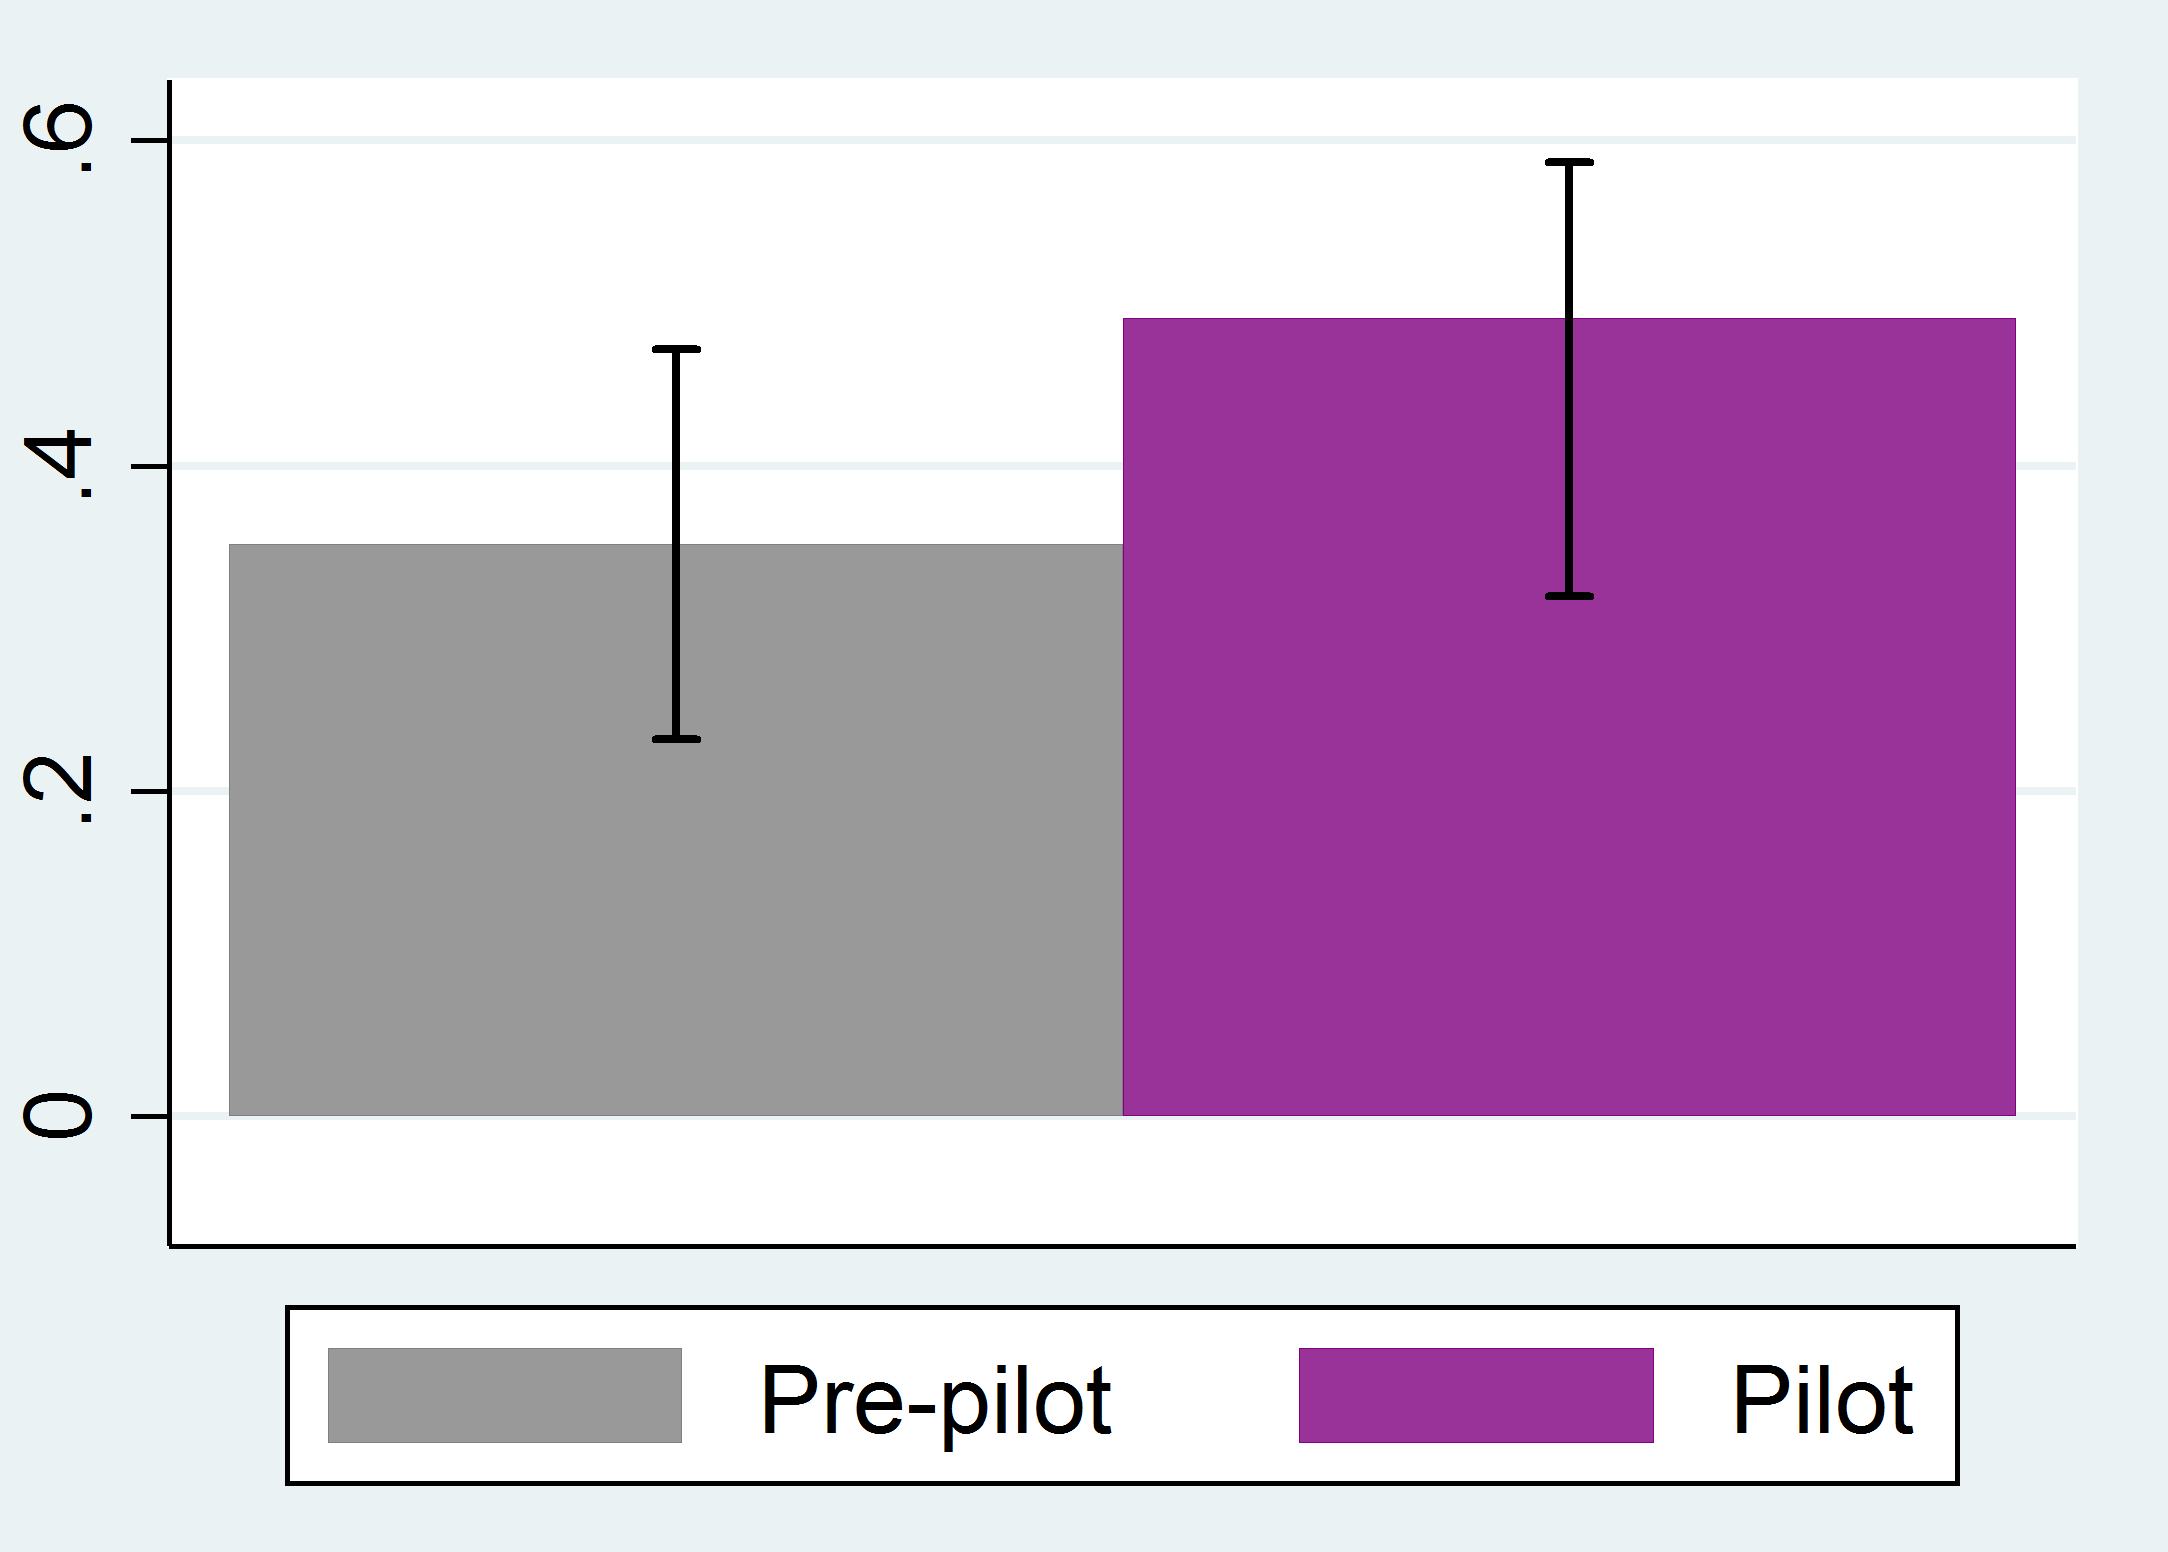
\includegraphics[width=0.7\linewidth]{../Raw/take_up}
			\caption{}
			\label{fig:take_up}
		\end{figure}
		\end{Verbatim}
	\end{center}
	
	Note that the relative file path to your \emph{Raw} folder was created in end of this line:
	
	\begin{Verbatim}
	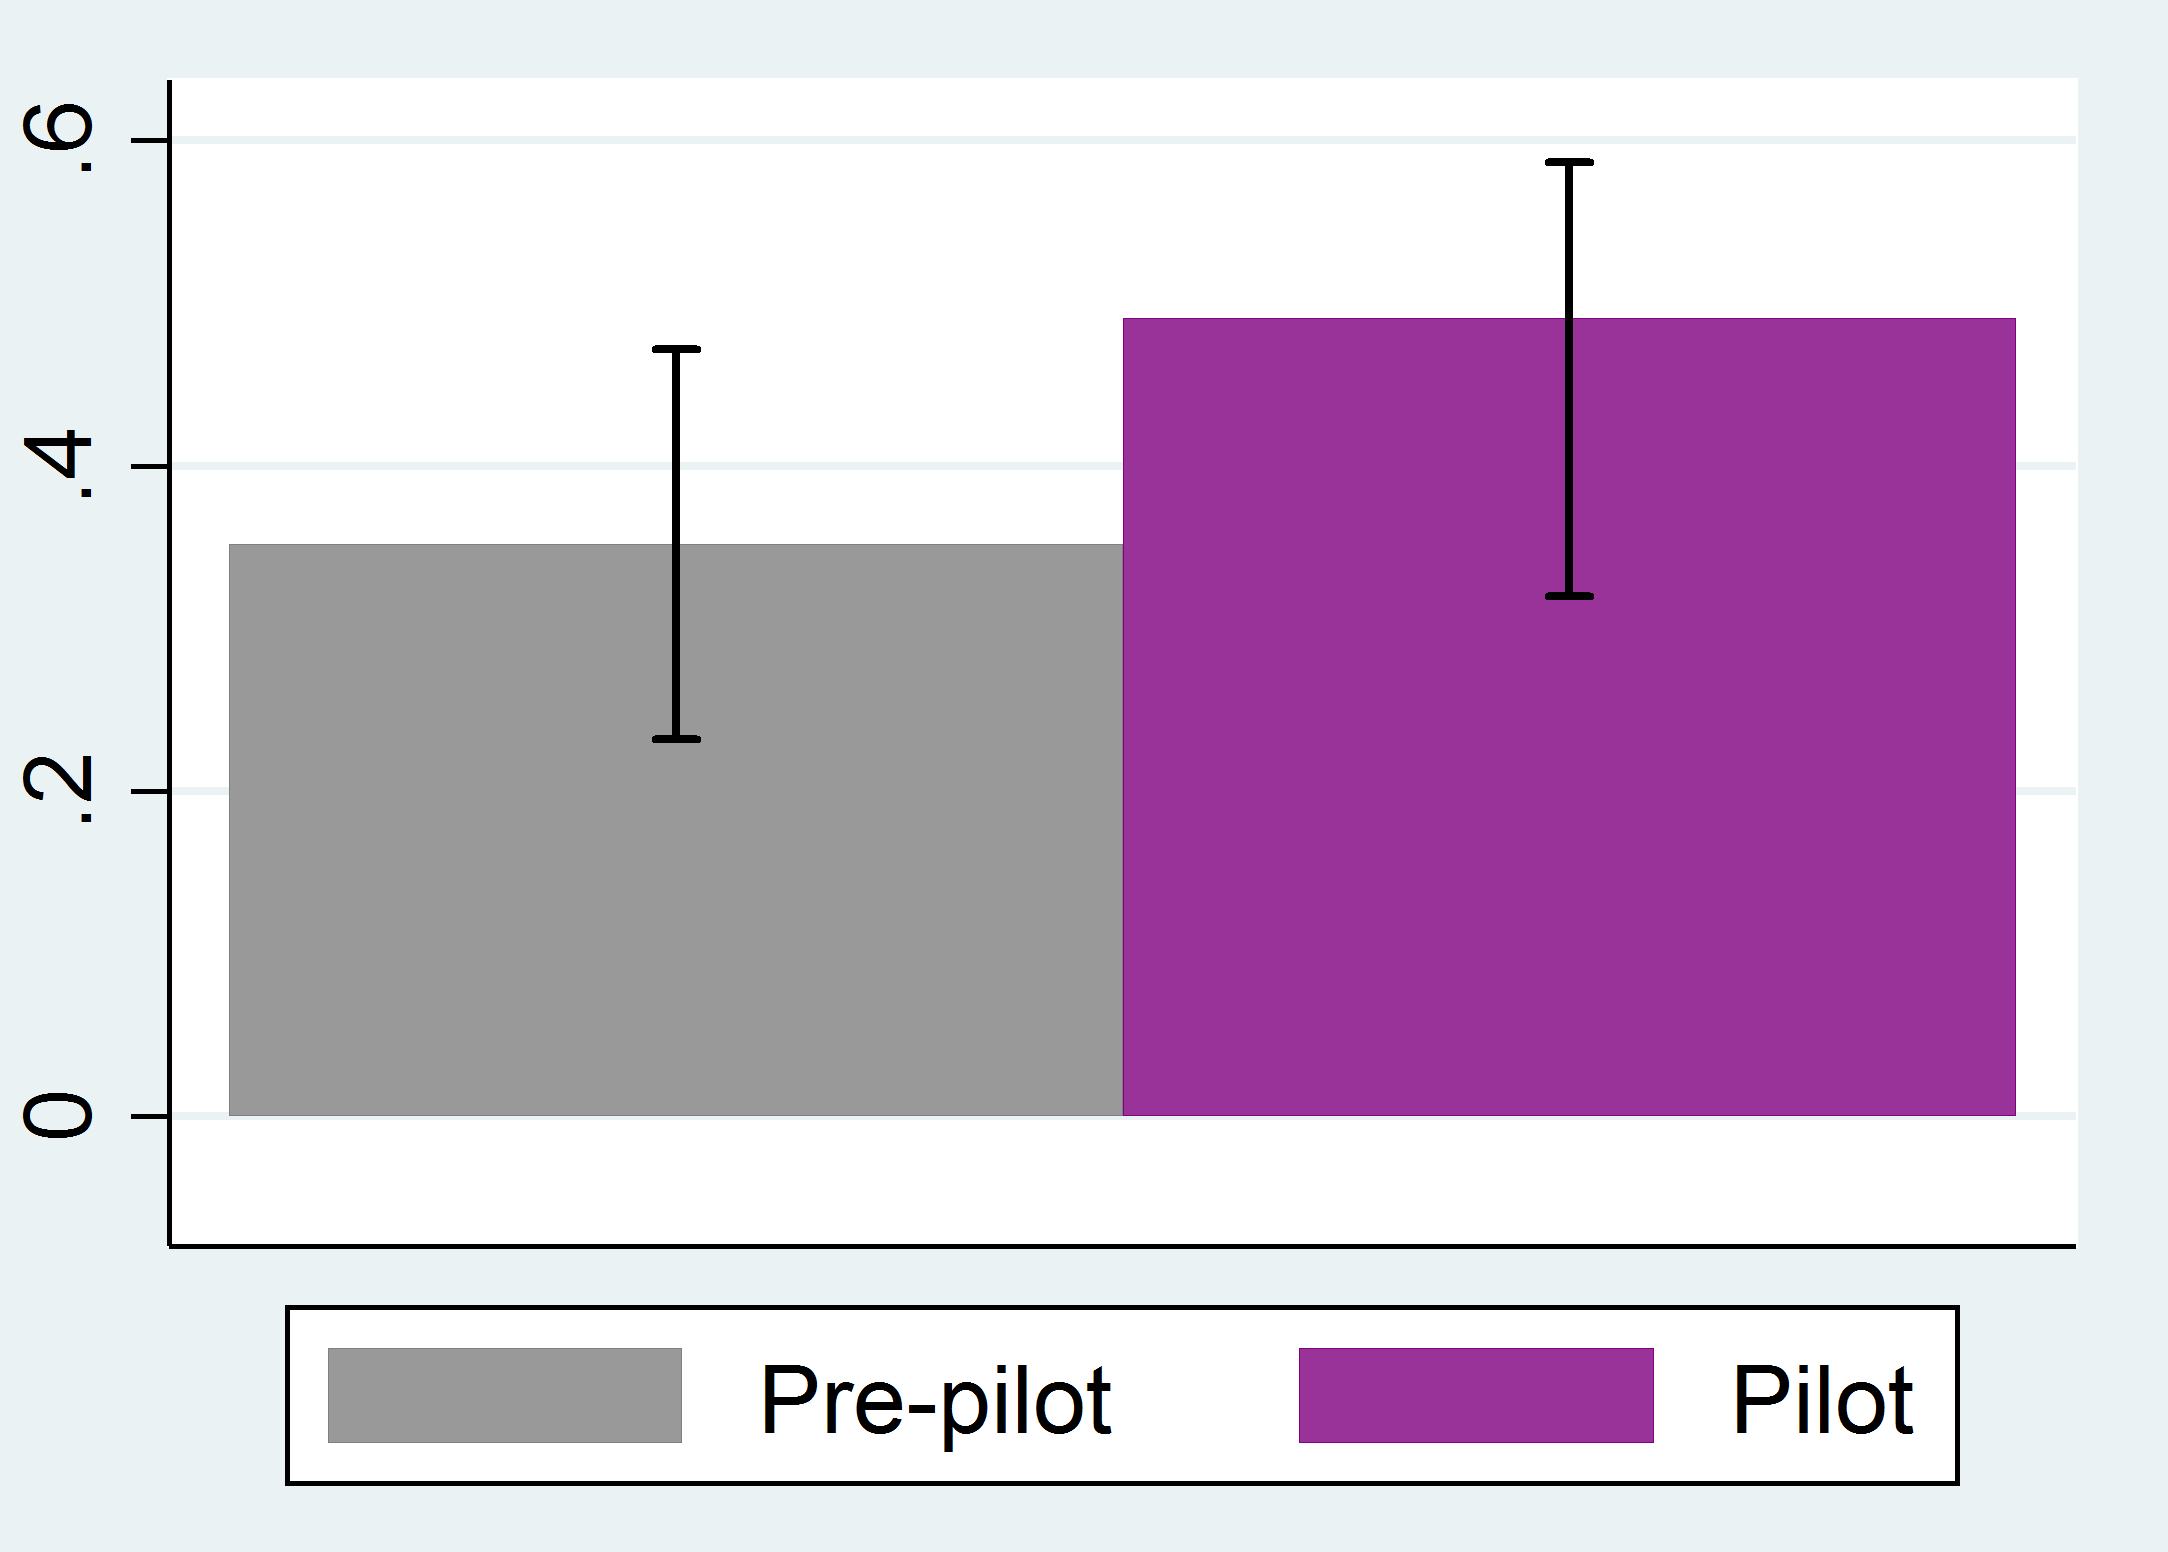
\includegraphics[width=0.7\linewidth]{../Raw/take_up}
	\end{Verbatim}
	
	In this example, the relative file path is \verb|{../Raw/take_up}|
	Note that the file extension is needed. You will see \verb|\begin{}| and \verb|\end{}| a lot in {\LaTeX}. The define where one object start and end, and the lines of code in between \verb|\begin{}| and \verb|\end{}| is called an environment. In the example above it is a figure environment. This tells {\LaTeX} that you are importing a figure and any other code in that environment in addition to the line with the relative path to the figure is a setting or provide some meta information to that figure. You will learn what \verb|\centering| and \verb|\caption{}| below. \verb|\label{fig:take_up}| is a slightly more advanced option and we will explore it on \emph{Exercise 2}. 
	
	\section{Manually importing graphs into \LaTeX}
	
	While click-and-drag is helpful to get started, you need to learn how to import figures and tables manually to {\LaTeX}. So now we want to manually import a second figure to your document. This will help us understand the functions of the other lines of code that TeXstudio created for us in the click-and-drag example.
	
	\textbf{Task 1:} Below the code that was generated when you imported the first figure (but before \verb|\end{document}|), create a figure environment and import \emph{iegraph.png} into it. You will find that graph in the \emph{Raw} folder. You import that figure by typing the following lines of code:
	
	\begin{center}
		\begin{Verbatim}[commandchars=+\(\)]
		\begin{figure}[H]
			\includegraphics{+color(CornflowerBlue)../Raw/+color(black)iegraph.png}
		\end{figure}
		\end{Verbatim}
	\end{center}
	
	Remember to include \color{CornflowerBlue}{\verb|../Raw/|}\color{black}{} as this is the relative path to the \emph{Raw} folder where \emph{regular\_graph.png} is saved. Compile your document. How does it look? 
	
	\textbf{Task 2:} We need to adjust the size of your figure so it fits into the page. Use the \verb|\width| option of \verb|\includegraphics{}| to do this by typing the context in blue:
	
	\begin{center}
		\begin{Verbatim}[commandchars=+\(\)]
		\begin{figure}[H]
			\includegraphics+color(CornflowerBlue)([width=\textwidth])+color(black)({../Raw/iegraph.png})
		\end{figure}
		\end{Verbatim}
	\end{center}
	
	The property \color{CornflowerBlue}{\verb|=\textwidth|}\color{black}{} means that the figure will be as wide as the margins of the text in your document. There are more properties that can be used with \verb|\width|, and you will learn more about these in later exercises, but for now, you can keep using only \verb|=\textwidth| for all figures and tables where it is necessary.
	
	\textbf{Task 3:} Add a title to your figure using the \verb|\caption| command:
	
	\begin{minipage}{\textwidth}
	\begin{center}
		\begin{Verbatim}[commandchars=+\(\)]
		\begin{figure}[H]
			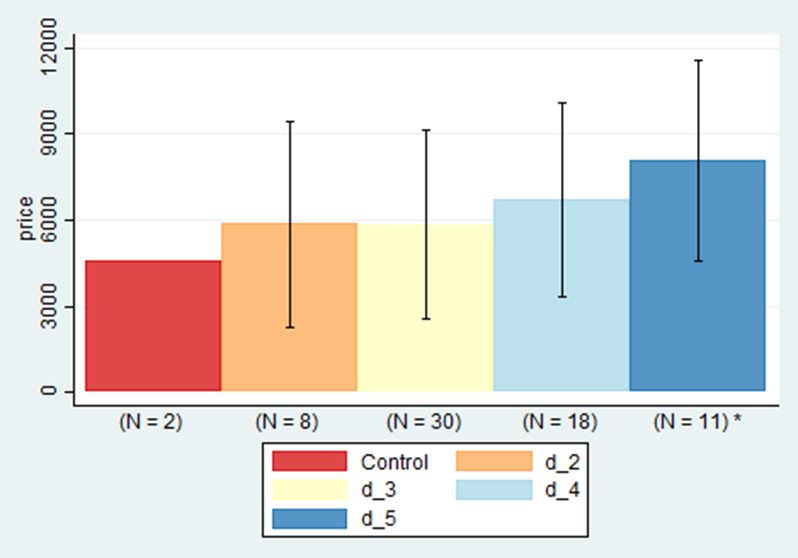
\includegraphics[width=\textwidth]{../Raw/iegraph.png}
			+color(CornflowerBlue)\caption{Add figure title here}
		\end{figure}
		\end{Verbatim}
	\end{center}
	\end{minipage}
	
	Change the caption from \verb|{Add figure title here}| to any title of your choice and compile the document again.
	
	\section*{Part 5. Importing tables into \LaTeX}
	\textbf{Task 1:} Create a table environment by using \verb|\begin{}| and \verb|\end{}| underneath the two figures you already imported. Instead of writing \verb|figure| in \verb|\begin{}| and \verb|\end{}| as you did above, write \verb|table|. This tells {\LaTeX} to expect a table instead if a figure. Import \emph{regression\_table.tex} into the table environment using \verb|\input{}|. This can be done by typing the following lines:
	
	\begin{center}
		\begin{Verbatim}[commandchars=+\(\)]
		\begin{table}[H]
			{
\def\sym#1{\ifmmode^{#1}\else\(^{#1}\)\fi}
\begin{tabular}{l*{8}{c}}
\hline\hline
                    &\multicolumn{1}{c}{(1)}&\multicolumn{1}{c}{(2)}&\multicolumn{1}{c}{(3)}&\multicolumn{1}{c}{(4)}&\multicolumn{1}{c}{(5)}&\multicolumn{1}{c}{(6)}&\multicolumn{1}{c}{(7)}&\multicolumn{1}{c}{(8)}\\
                    
\hline
Post        &      -0.304\sym{*}  &      -0.632\sym{***}&       0.003         &       0.217\sym{**} &      -0.059         &      -0.012         &       0.136         &       0.333         \\
                    &     (0.141)         &     (0.026)         &     (0.130)         &     (0.072)         &     (0.082)         &     (0.029)         &     (0.365)         &     (0.265)         \\
[1em]
Treatment     &      -0.055         &       0.267\sym{***}&      -0.133\sym{*}  &       0.096         &      -0.210\sym{*}  &      -0.035         &      -0.117         &      -0.033\sym{***}\\
                    &     (0.152)         &     (0.000)         &     (0.064)         &     (0.105)         &     (0.098)         &     (0.078)         &     (0.133)         &     (0.000)         \\
[1em]
Post * treatment &               &               &       0.065         &      -0.254\sym{*}  &       0.111         &      -0.000         &       0.284         &      -0.585         \\
                    &                 &                &     (0.159)         &     (0.116)         &     (0.086)         &     (0.033)         &     (0.378)         &     (0.296)         \\
[1em]
Constant            &       0.581\sym{***}&       0.333\sym{***}&       0.378\sym{***}&       0.175         &       0.276\sym{**} &       0.039         &       0.364\sym{**} &       0.000         \\
                    &     (0.131)         &     (0.000)         &     (0.055)         &     (0.105)         &     (0.095)         &     (0.081)         &     (0.115)         &     (0.000)         \\
\hline
Observations        &         354         &         354         &        1897         &        1897         &        1652         &        1652         &         348         &         348         \\
Fixed-effects  &          No         &         Yes         &          No         &         Yes         &          No         &         Yes         &          No         &         Yes         \\

\(R^{2}\)           &       0.033         &       0.595         &       0.014         &       0.287         &       0.043         &       0.386         &       0.076         &       0.535         \\

\hline\hline
\multicolumn{9}{l}{\footnotesize Standard errors clustered at user level are in parentheses. \sym{*} \(p<0.05\), \sym{**} \(p<0.01\), \sym{***} \(p<0.001\)}\\
\end{tabular}
}

		\end{table}
		\end{Verbatim}
	\end{center}
	
	Compile the document and look at the table. 
	
	\textbf{Task 2:} We need to adjust the size of the table. When we are using \verb|\input{}|, we have to do that slightly differently to how we did it for \emph{iegraph.png} above. Use \verb|\adjustBox| to adjust table size. Everything added between \verb|\begin{adjustbox}| and \verb|\end{adjustbox}| will have the property \verb|{max width=\textwidth}|. See the code in blue below:
	
	\begin{center}
		\begin{Verbatim}[commandchars=+\(\)]
		\begin{table}[H]
			+color(CornflowerBlue)(\begin{adjustbox}{max width=\textwidth})  
			{
\def\sym#1{\ifmmode^{#1}\else\(^{#1}\)\fi}
\begin{tabular}{l*{8}{c}}
\hline\hline
                    &\multicolumn{1}{c}{(1)}&\multicolumn{1}{c}{(2)}&\multicolumn{1}{c}{(3)}&\multicolumn{1}{c}{(4)}&\multicolumn{1}{c}{(5)}&\multicolumn{1}{c}{(6)}&\multicolumn{1}{c}{(7)}&\multicolumn{1}{c}{(8)}\\
                    
\hline
Post        &      -0.304\sym{*}  &      -0.632\sym{***}&       0.003         &       0.217\sym{**} &      -0.059         &      -0.012         &       0.136         &       0.333         \\
                    &     (0.141)         &     (0.026)         &     (0.130)         &     (0.072)         &     (0.082)         &     (0.029)         &     (0.365)         &     (0.265)         \\
[1em]
Treatment     &      -0.055         &       0.267\sym{***}&      -0.133\sym{*}  &       0.096         &      -0.210\sym{*}  &      -0.035         &      -0.117         &      -0.033\sym{***}\\
                    &     (0.152)         &     (0.000)         &     (0.064)         &     (0.105)         &     (0.098)         &     (0.078)         &     (0.133)         &     (0.000)         \\
[1em]
Post * treatment &               &               &       0.065         &      -0.254\sym{*}  &       0.111         &      -0.000         &       0.284         &      -0.585         \\
                    &                 &                &     (0.159)         &     (0.116)         &     (0.086)         &     (0.033)         &     (0.378)         &     (0.296)         \\
[1em]
Constant            &       0.581\sym{***}&       0.333\sym{***}&       0.378\sym{***}&       0.175         &       0.276\sym{**} &       0.039         &       0.364\sym{**} &       0.000         \\
                    &     (0.131)         &     (0.000)         &     (0.055)         &     (0.105)         &     (0.095)         &     (0.081)         &     (0.115)         &     (0.000)         \\
\hline
Observations        &         354         &         354         &        1897         &        1897         &        1652         &        1652         &         348         &         348         \\
Fixed-effects  &          No         &         Yes         &          No         &         Yes         &          No         &         Yes         &          No         &         Yes         \\

\(R^{2}\)           &       0.033         &       0.595         &       0.014         &       0.287         &       0.043         &       0.386         &       0.076         &       0.535         \\

\hline\hline
\multicolumn{9}{l}{\footnotesize Standard errors clustered at user level are in parentheses. \sym{*} \(p<0.05\), \sym{**} \(p<0.01\), \sym{***} \(p<0.001\)}\\
\end{tabular}
}

			+color(CornflowerBlue)(\end{adjustbox})
		\end{table}
		\end{Verbatim}
	\end{center}
	
	\textbf{Task 3:} Similar to figures, you can add a caption to your table. This is done by adding the same lines as for figures.
	
	\begin{minipage}{\textwidth}
	\begin{center}
		\begin{Verbatim}[commandchars=+\(\)]
		\begin{table}[H]
			+color(CornflowerBlue)\caption{Add a title to this table}
			\begin{adjustbox}{max width=\textwidth}
				{
\def\sym#1{\ifmmode^{#1}\else\(^{#1}\)\fi}
\begin{tabular}{l*{8}{c}}
\hline\hline
                    &\multicolumn{1}{c}{(1)}&\multicolumn{1}{c}{(2)}&\multicolumn{1}{c}{(3)}&\multicolumn{1}{c}{(4)}&\multicolumn{1}{c}{(5)}&\multicolumn{1}{c}{(6)}&\multicolumn{1}{c}{(7)}&\multicolumn{1}{c}{(8)}\\
                    
\hline
Post        &      -0.304\sym{*}  &      -0.632\sym{***}&       0.003         &       0.217\sym{**} &      -0.059         &      -0.012         &       0.136         &       0.333         \\
                    &     (0.141)         &     (0.026)         &     (0.130)         &     (0.072)         &     (0.082)         &     (0.029)         &     (0.365)         &     (0.265)         \\
[1em]
Treatment     &      -0.055         &       0.267\sym{***}&      -0.133\sym{*}  &       0.096         &      -0.210\sym{*}  &      -0.035         &      -0.117         &      -0.033\sym{***}\\
                    &     (0.152)         &     (0.000)         &     (0.064)         &     (0.105)         &     (0.098)         &     (0.078)         &     (0.133)         &     (0.000)         \\
[1em]
Post * treatment &               &               &       0.065         &      -0.254\sym{*}  &       0.111         &      -0.000         &       0.284         &      -0.585         \\
                    &                 &                &     (0.159)         &     (0.116)         &     (0.086)         &     (0.033)         &     (0.378)         &     (0.296)         \\
[1em]
Constant            &       0.581\sym{***}&       0.333\sym{***}&       0.378\sym{***}&       0.175         &       0.276\sym{**} &       0.039         &       0.364\sym{**} &       0.000         \\
                    &     (0.131)         &     (0.000)         &     (0.055)         &     (0.105)         &     (0.095)         &     (0.081)         &     (0.115)         &     (0.000)         \\
\hline
Observations        &         354         &         354         &        1897         &        1897         &        1652         &        1652         &         348         &         348         \\
Fixed-effects  &          No         &         Yes         &          No         &         Yes         &          No         &         Yes         &          No         &         Yes         \\

\(R^{2}\)           &       0.033         &       0.595         &       0.014         &       0.287         &       0.043         &       0.386         &       0.076         &       0.535         \\

\hline\hline
\multicolumn{9}{l}{\footnotesize Standard errors clustered at user level are in parentheses. \sym{*} \(p<0.05\), \sym{**} \(p<0.01\), \sym{***} \(p<0.001\)}\\
\end{tabular}
}

			\end{adjustbox}
		\end{table}
		\end{Verbatim}
	\end{center}
	\end{minipage}
	
	Update the text in \verb|\caption{Add figure title here}| and compile the document. See that the title of the table is above the table. When we used \verb|\caption{}| for the figure earlier the title was below the table. That has nothing to do with tables and figures, it all depends if you enter the line with \verb|\caption{}| before or after the line when you are importing a file to your document. To test this, move the line with the caption to after \verb|\end{adjustbox}| and before \verb|\end{table}|, and compile the document again. Note that the caption line must come before the adjustbox environment begins, otherwise the document will not compile.
	
	\section{Centering imported objects}
	Until now, we imported object into our document that were too wide for our document margins, so we had to adjust their sizes. Next, we are going to see what happens when you import a narrower object. To do this, create a table environment, import and create a title for the table in \emph{sampl\_sizes.tex}. This table can also be found in the \emph{Raw} folder:
	
	\begin{center}
		\begin{Verbatim}[commandchars=+\(\)]
		\begin{table}[H]
			\caption{Add a title to this table}
			{
\def\sym#1{\ifmmode^{#1}\else\(^{#1}\)\fi}
\begin{tabular}{l*{4}{c}}
\hline\hline
          &\multicolumn{1}{c}{Group 1}&\multicolumn{1}{c}{Group 2}&\multicolumn{1}{c}{Group 3}&\multicolumn{1}{c}{Group 4}\\
\hline
Control   &       203         &       945         &        700         &        200         \\
Treatment &       151         &       952         &        952         &        148         \\
\hline
Total     &       354         &       1897         &       1652         &       348         \\
\hline\hline
\end{tabular}
}

		\end{table}
		\end{Verbatim}
	\end{center}
	
	As you can see, this table is not yet centered, but we can fix that by adding one line to its environment:
	
	\begin{center}
		\begin{Verbatim}[commandchars=+\(\)]
		\begin{table}[H]
			+color(CornflowerBlue)\centering
			\caption{Add a title to this table}
			{
\def\sym#1{\ifmmode^{#1}\else\(^{#1}\)\fi}
\begin{tabular}{l*{4}{c}}
\hline\hline
          &\multicolumn{1}{c}{Group 1}&\multicolumn{1}{c}{Group 2}&\multicolumn{1}{c}{Group 3}&\multicolumn{1}{c}{Group 4}\\
\hline
Control   &       203         &       945         &        700         &        200         \\
Treatment &       151         &       952         &        952         &        148         \\
\hline
Total     &       354         &       1897         &       1652         &       348         \\
\hline\hline
\end{tabular}
}

		\end{table}
		\end{Verbatim}
	\end{center}
	
	Adding \verb|\centering| to the beginning of an environment centers whatever is in that environment. That means that if the same line was added after a \verb|\begin{figure}|, that figure would also be centered.
	
	
	\section{Adding a document title}
	We are almost done with this document now but so far we only have tables and figures. In this part we want to add a title to the document and in the next part we will add a list of tables and a list of figures. All of these are very easy to set up.
	
	To add a title to your document, add \verb|\maketitle| on a new line immediately below \verb|\begin{document}|. Compile the document. You can see the information we already added. Update this information with a title of your own and with you name in the preamble. Look for this section and update the text that is blue below.
	
	\begin{center}
		\begin{Verbatim}[commandchars=+\(\)]
+color(Gray)% ADD YOUR PROJECT INFO HERE 
\title{+color(CornflowerBlue)DIME template for \LaTeX \\ Importing tables+color(black)}    +color(Gray)% Double backslash starts a new line
\author{+color(CornflowerBlue)Luiza Andrade \& Mrijan Rimal+color(black)}
\date{}                                              +color(Gray)% Updates and prints date automatically
		\end{Verbatim}
	\end{center}
	
	\section{Add a list of tables and a list of figures}
	Finally we want to create a list of tables and figures that is automatically updated if you were to add or remove tables and figures. Immediately after where you added \verb|\maketitle|, on a new line, add \verb|\listoftables| and, on a second new line, add \verb|\listoffigures|. Like this:

	\begin{center}
		\begin{Verbatim}[commandchars=+\(\)]
		\begin{document}
		\maketitle
		\listoftables
		\listoffigures
		\end{Verbatim}
	\end{center}
	
	Compile your document. The titles shown in these lists are those defined by the \verb|\caption| you added to each table and figure. Go to any of your figures or tables and change the caption and compile the document again. See how the list of tables and figures is updated. While it is common practice, you do not need to add \verb|\maketitle| and \verb|\listoftables| in the beginning of the document. You can add them anywhere.

	
\end{document}         